%%%% ijcai17.tex

\typeout{IJCAI-17 Instructions for Authors}

% These are the instructions for authors for IJCAI-17.
% They are the same as the ones for IJCAI-11 with superficical wording
%   changes only.

\documentclass{article}
% The file ijcai17.sty is the style file for IJCAI-17 (same as ijcai07.sty).
\usepackage{ijcai17}

% Use the postscript times font!
\usepackage{times}

% the following package is optional:
%\usepackage{latexsym} 

% Following comment is from ijcai97-submit.tex:
% The preparation of these files was supported by Schlumberger Palo Alto
% Research, AT\&T Bell Laboratories, and Morgan Kaufmann Publishers.
% Shirley Jowell, of Morgan Kaufmann Publishers, and Peter F.
% Patel-Schneider, of AT\&T Bell Laboratories collaborated on their
% preparation.

% These instructions can be modified and used in other conferences as long
% as credit to the authors and supporting agencies is retained, this notice
% is not changed, and further modification or reuse is not restricted.
% Neither Shirley Jowell nor Peter F. Patel-Schneider can be listed as
% contacts for providing assistance without their prior permission.

% To use for other conferences, change references to files and the
% conference appropriate and use other authors, contacts, publishers, and
% organizations.
% Also change the deadline and address for returning papers and the length and
% page charge instructions.
% Put where the files are available in the appropriate places.


% added pakages
\usepackage{epsfig} %% for loading postscript figures
\usepackage{subcaption}





\title{Community detection and analysis with trajectory history of taxi drivers}
\author{Carles Sierra\\ 
Artificial Intelligence Research Institute, IIIA-CSIC, Bellaterra, Catalonia  \\
pcchair@ijcai-17.org}

\begin{document}

\maketitle

\begin{abstract}
  The {\it IJCAI--17 Proceedings} will be printed from electronic
  manuscripts submitted by the authors. The electronic manuscript will
  also be included in the online version of the proceedings. This paper
  provides the style instructions.
\end{abstract}

\section{Introduction} \label{sec:introduction}

It is natural that people find and form a community to share information. They get benefits from others, and they also contribute to the community. Active communities communicate with members often and achieve their goals. However, some others consist of people who have the similar preference but just flock together. This results from homophily, love of the same. In this research, we aim to quantify interaction in a community and to detect active communities.In taxi industry, drivers share information such as locations where they can easily pick up passengers without long queueing time. It means that there is community structure in taxi driver's network. However, it is difficult to find communities without drivers' contact list, and the list does not necessarily mean real communities.

The advanced information technology collects all data from anywhere and at any time. In the case of the taxi industry, vehicles' information such as position and speed is regularly recorded, which constitutes trajectory history. Whenever a driver picks up and drop off a passenger, servers store locations, fare, duration, etc.. This information makes us overcome the challenge mentioned before.

The massive trajectory data generated by moving objects such as people, animal and vehicles gives us opportunities to understand behavior of objects and to utility that knowledge. Zheng~\shortcite{Zheng2015} summarizes various trajectory data mining research and, especially, introduces several trajectory pattern mining research. They are aim to find a group of objects that shows move together or similar patterns. One of applications is recommendation systems. Some researches define the similarity between users with trajectory history \cite{Xiao2014,Liu2016}. Xiao et al.~\shortcite{Xiao2014} focuses on semantic location, not just physical locations, and manipulate an information retrieval method, TF-IDF (term frequency-inverse document frequency). Liu and Wang~\shortcite{Liu2016} tries to get more accurate similarity score. Not only consider locations, but this research also include factors such as temporal duration, spatial proximity to other objects and movement velocity. The research related to recommendation systems can also find a group of people and groups. However our interest is active communities. A community is a group of people but a group does not necessarily means a community in terms of homophily and influence between members.

Some researches have more interests in influence between people. Shimizu~\shortcite{Shimizu2008} propose a Viral Diffusion Model to capture information flows in a community. This research use a mailing list data and measures the impact of users' comment by comparing similarity in subsequent comments. Song et al.~\shortcite{Song2010} also focuses on communication between users. It quantifies relationship through Weighted Harmonic Rule which includes the intensity of the conversation. Arel et al.~\shortcite{Aral2009} explicitly distinguishes peer influence and homophily effect. With sampling and statistics approach, this research quantifies peer influence in product adoption decisions.

Many community detection researches mainly focus on how to partition a given graph into subgraphs. Planti{\'e} and Crampes~\shortcite{Plantie2013} introduces many community detection algorithm and says that modularity has been used by many researchers to measure the performance of a community detection algorithm. This is because high values in modularity means there are many intra-community edges but few edges between different communities. Blondel et al.~\shortcite{Blondel2008} directly uses modularity with a heuristic approach, which iteratively merges communities if the mergence gives a better modularity value. Steinhaeuser and Chawla~\shortcite{Steinhaeuser2008} and Expert et al.~\shortcite{Expert2011} also use modularity in algorithms, but they modifies it depending on problems they focuses. Chen et al.~\shortcite{Chen2011} models a community detection problem using game theory. In this research, agents can choose communities, a gain function is modularity and Nash equilibriums represents community structures.

In this research, we quantify drivers' influence to other drivers with a linear regression model, build weighted directed graphs and applies the well-known partition algorithm to detect communities. Furthermore, we compare some statistics of communities and validate our framework by another regression model that estimates locations where members in the same community share. A challenge in this work is that we do not have prior information about drivers' contact list. Also, to find active communities, we need to exclude homophily effect in a systematic way. The remainder of this research is organized as follows. In Section~\ref{sec:background}, we introduce background about taxi industry and dataset. In Section~\ref{sec:comDectectionFramework}, our framework is explained in detail. In Section 4, we show our results and validate them in another perspective. Lastly, we summarize our research and conclude with discussions.


\section{Background} \label{sec:background}

In big data era, collecting data is common to analyze and to utilize it in the future. The taxi industry has also been trying to get knowledge from data. The dataset we use in this research is provided by a taxi company in Singapore from 2009 to 2012. Every 45$\sim$50 seconds, equipment in a vehicle logs taxi's GPS coordinates, speed and state such as free and passenger on board. These logs are saved in a file and the size of the file about a month is around 15$\sim$20 GB. When a driver picks up and drops off a passenger, additional information such as fare and trip duration is also recorded. We name a file which includes these information as trip dataset. Basically, each file has records about a month and the number of trip instances in a month is around 11$\sim$12 millions. The number of all taxi drivers considered is more 34 thousand, they work 7.7 hours and earn S\$ 194.5 in a day on average.


\begin{figure} [h] 

\centering
\begin{subfigure}{\linewidth}
  \centering
  \includegraphics[width=0.95\linewidth]{figs/gridSingapore}
  \caption{Grid form}
  \label{fig:gridSingapore}
\end{subfigure}

\begin{subfigure}{\linewidth}
  \centering
  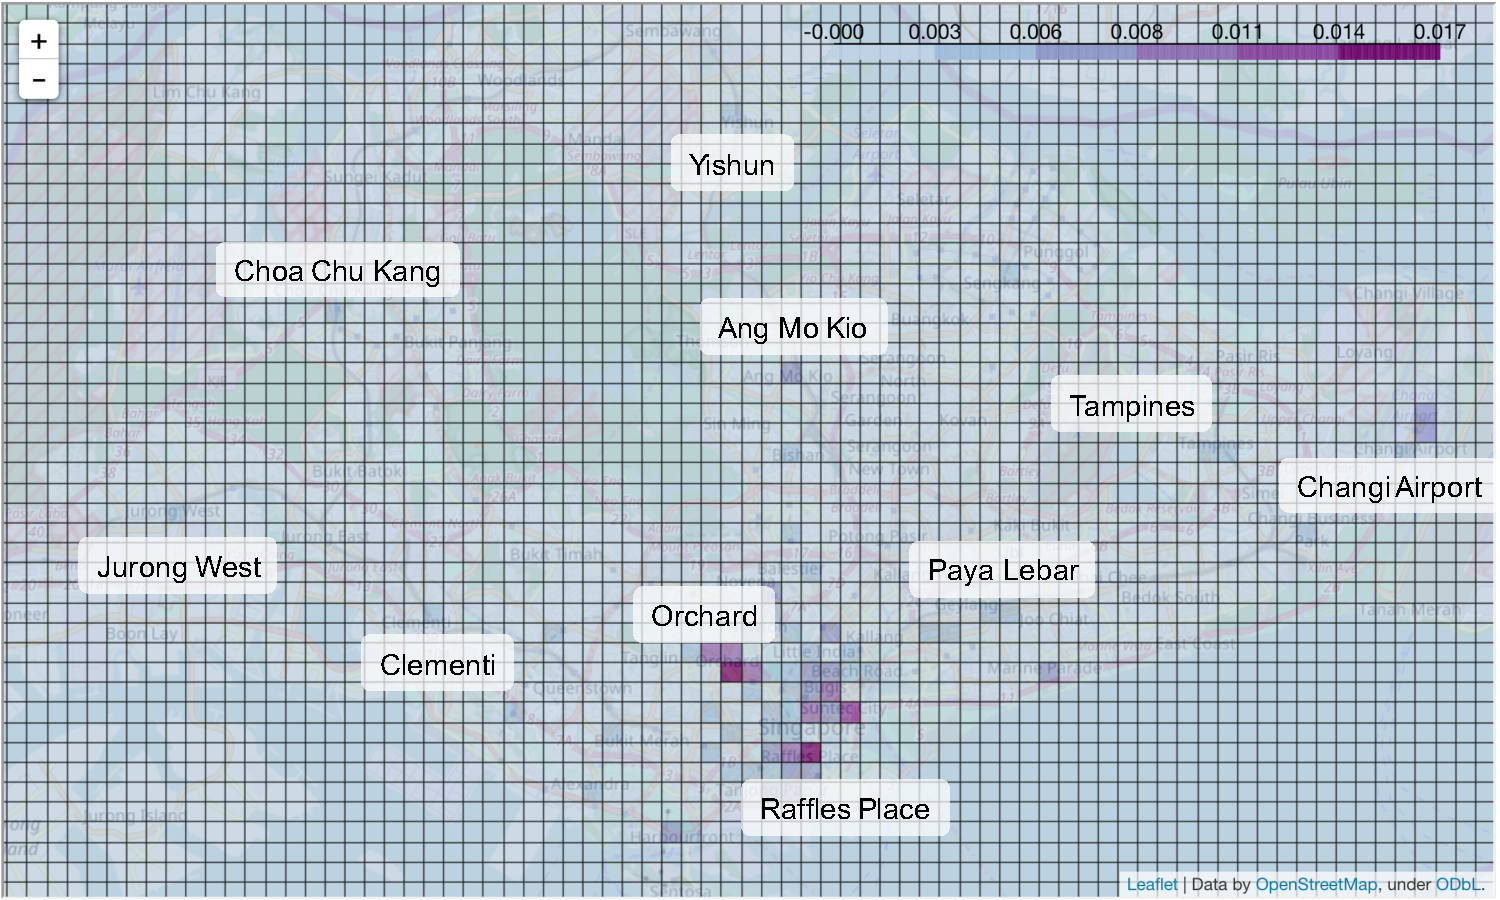
\includegraphics[width=0.95\linewidth]{figs/locationHeatMap}
  \caption{Pick-up location heat map}
  \label{fig:locationHeatMap}
\end{subfigure}

%\vspace{-0.3 cm}
\caption{Map of Singapore}
\label{fig:mapSingapore}
%\vspace{-0.5 cm}
\end{figure}


We split Singapore in a grid form, like Figure~\ref{fig:gridSingapore}, to manage trajectory history efficiently and define each cell as zones. The size of a cell is 0.5km by 0.5km. We consider that this size is enough to capture queueing time. Queueing time is defined roaming time for finding a passenger or waiting at a taxi stand. More details about quantifying queueing time are mentioned in Section~\ref{sec:comDectectionFramework}. Figure~\ref{fig:locationHeatMap} shows general locations where taxi drivers pick up passengers often. Most of the trips occurred at city areas such as Orchard and Raffles Place. Removing homophily effect is a big issue in detecting active community. For example, many last mile trips, from a transportation hub to a final destination, occurs in a few locations such as Yishun and Tampines. Some drivers usually return the same location where they pick up passengers after they finish services. They show same trajectory patterns, but it is hard to define them as the same community because they just follow their preference without interaction with other drivers. Therefore, we need a systematic approach to detect real and active communities.



\section{Community detection framework} \label{sec:comDectectionFramework}

The keys of our community detection framework are to handle drivers’ trajectory history, to quantify the relationships between drivers and to define communities that there are active communications between inner members. Figure~\ref{fig:frameworkOutline} shows our framework conceptually. Firstly, we define queueing time and find drivers who may have the relationship with a driver with trajectory history. In the second phrase, we construct a directed and weighted graph that represents driver's influence network by quantifying the relationships with a linear regression model with multiple variables. In the third phrase, we partition the graph and define communities. Lastly, we apply another regression model to discover zones where members of a community have interests.


\begin{figure} [h]
  \centering
  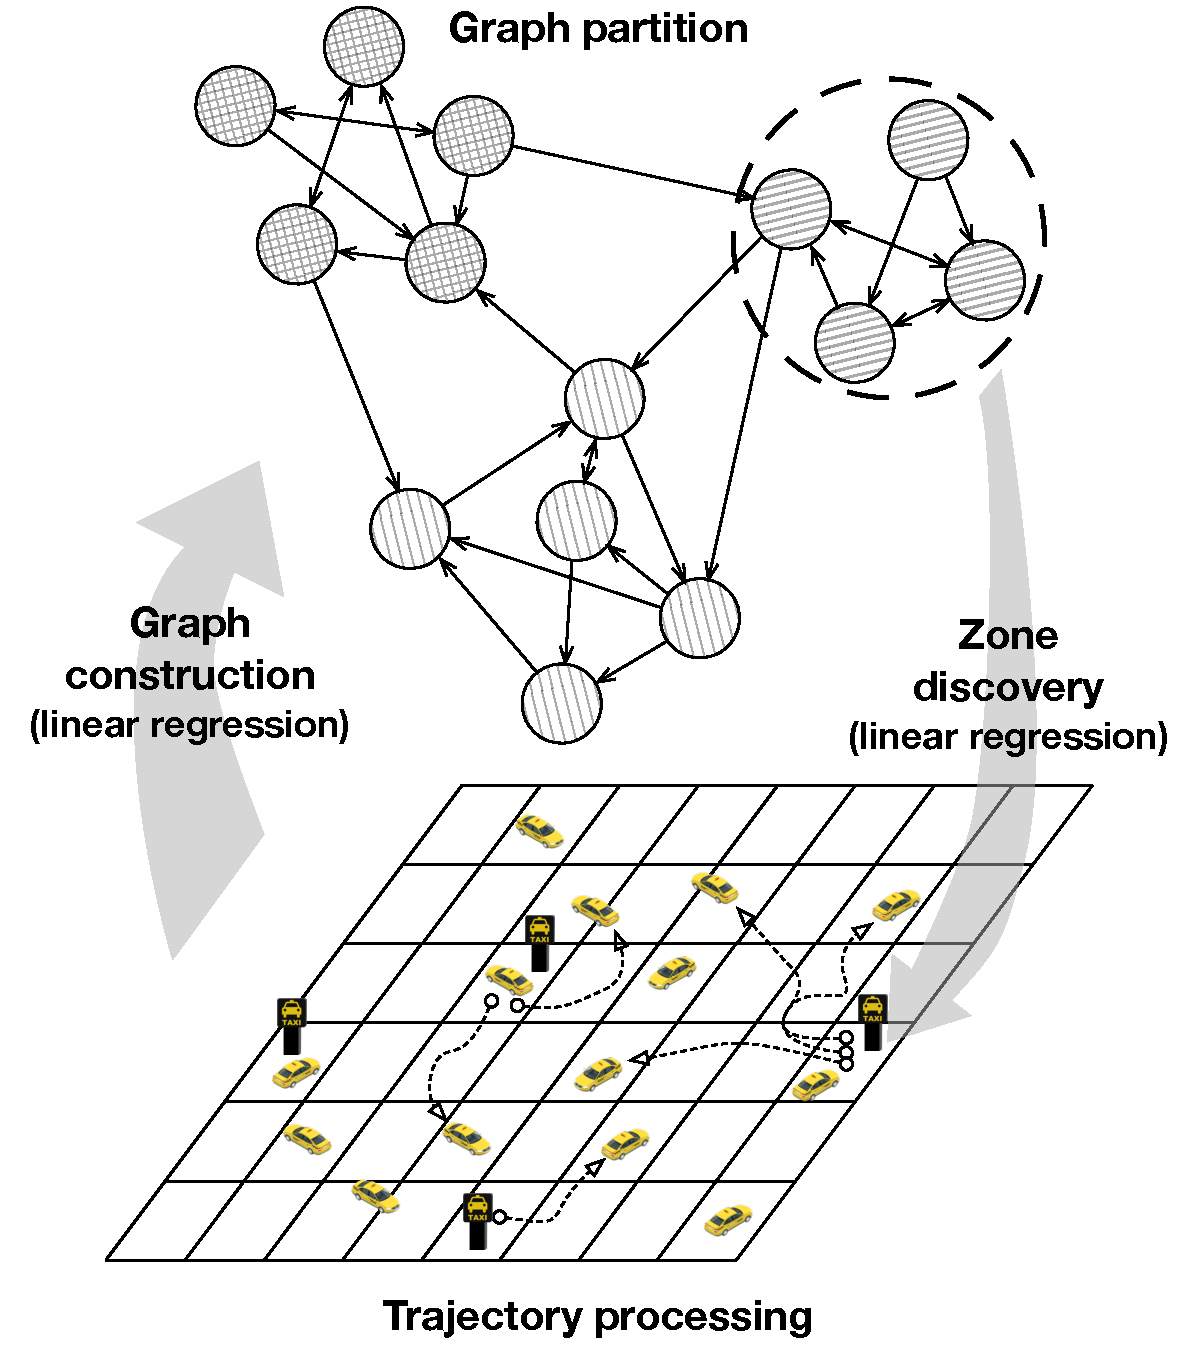
\includegraphics[width=.8\linewidth]{figs/frameworkOutline}
  \caption{Queueing time and previous drivers}
  \label{fig:frameworkOutline}
\end{figure}

We control taxi drivers and trip dataset to get reliable results. In Singapore, many drivers share vehicles with others and we regard that their relationship is not strong as that of single shift drivers who does not share the vehicle with others. There are 65$\sim$70 thousand drivers single shift drivers among the whole drivers. We only consider single shift drivers in this research because we have interests in active communities.  Another control attribute is about time and day of the week. During the rush hour, it is not like for drivers to communicate each other because they can easily find passengers. Even they get information from others, the drivers cannot go the location soon because of congestion. Few passengers wait for taxis and many drivers do not operate taxis in the middle of the night. Therefore, we ignore trip instances occurred from 0 AM ~ 2 PM. Also, because driving patterns on weekdays and weekends are very different, we focus on weekday's trips except for Friday whose trip pattern is different with that of other weekdays.


\subsection{Trajectory processing} \label{sec:traProcessing}

We consider queueing time as the measure that shows the influence of other drivers. Let's imagine a situation that a driver picks up a passenger at a zone where other passengers also wait for taxicabs. It is highly recommended for the driver to call other drivers if he has the close friendship with them. As a result, by going to the same zone, the driver who gets information from the previous driver can save time for finding a new passenger. For example in Figure~\ref{fig:QtimePrevDrivers}, the reason why driver $D_i$ go to the taxi stand is that driver $D_1$ give the information. Formally, we define queueing time as the interval between the time when a driver enter the zone where he picks up a passenger ($t_e$) and passenger pick-up time ($t_p$).

\begin{figure} [h]
  \centering
  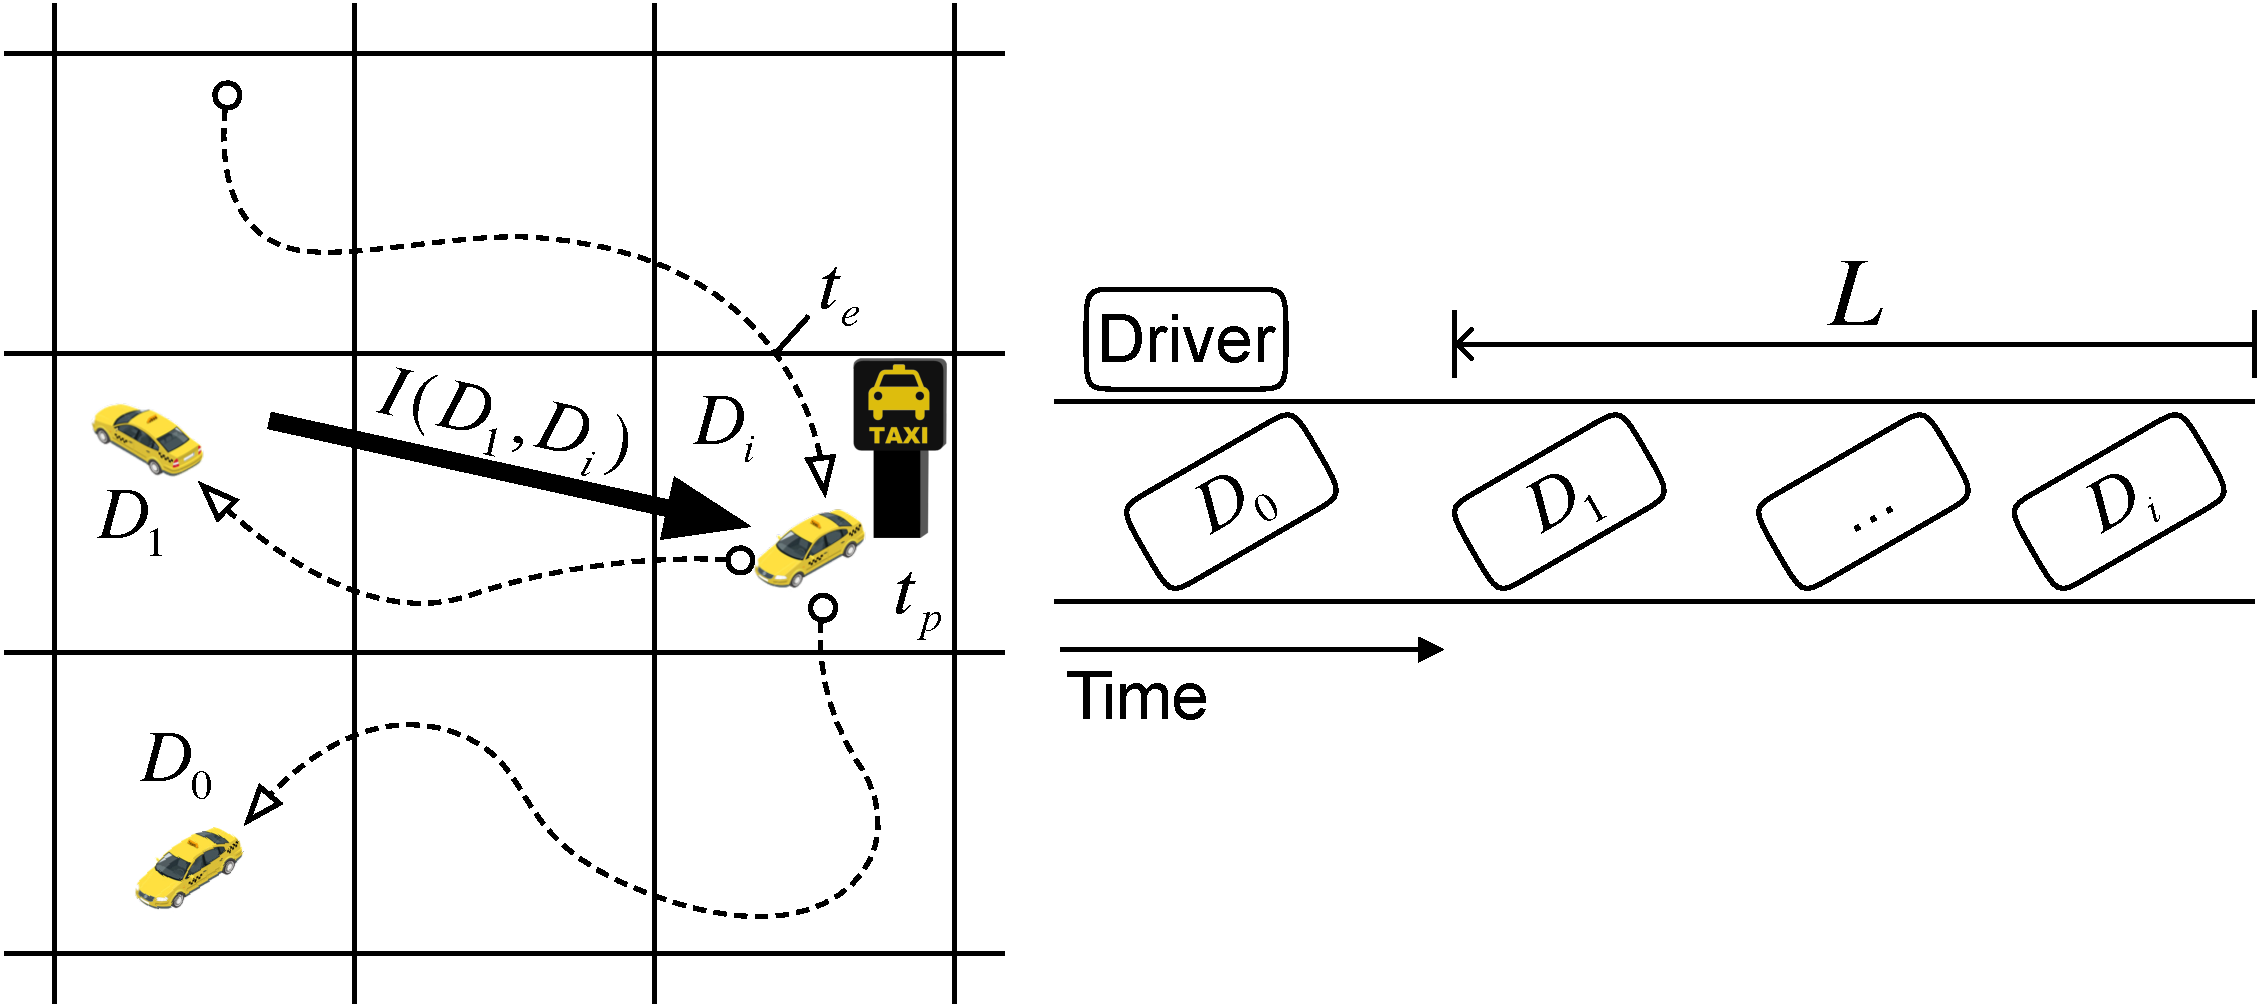
\includegraphics[width=1.0\linewidth]{figs/QtimePrevDrivers}
  \caption{Queueing time and previous drivers}
  \label{fig:QtimePrevDrivers}
\end{figure}

Because there are some errors in the empirical dataset, some outliers in terms of queueing time need to be discarded. It is general to use the mean and three standard deviation values for filtering outlier. However, this criteria cannot handle extremely skewed dataset like ours. Therefore we use 95 percentile value for filtering. 

The next thing to do is to find a driver who gives the information. There can be multiple drivers who pick up passengers at the same zone. Someones did it the long time ago, like $D_0$, others started services just ago. Here, we assume that if a driver received the information, he would appear in the zone within a certain time, $L$. We define drivers whose passenger pick-up time belong to $[t_{p}-L,t_{p}]$ as previous drivers, \emph{prevDrivers}. These drivers are highly likely to have the relationship with the driver who is picking up passenger now. However, it might be wrong that all previous drivers communicate with the driver. For example, if some popular sights are in the zone, many taxi driver will join the taxi stand, not because of communication. Therefore, in the next section, we suggest a regression model that removes the homophily effect and quantifies the influence of drivers, $I(D_i,D_j)$.

\subsection{Graph construction} \label{sec:graphConstruction}

Linear regression is a powerful tool in data analysis. We use this tool to quantify the influence of drivers by utilizing the meaning of coefficient. A coefficient has a meaning that the increment of dependent variable's one unit changes dependent variable as much as the coefficient. Especially, if a dependent variable is a binary value, the interpretation is more intuitive. We model our problem as a linear regression with multiple binary variables. A dependent variable is queuing time of a driver and independent variables prior presence of the previous drivers. Equation~\ref{eq:influenceRegression} shows driver $i$ 's regression model;

\begin{equation} \label{eq:influenceRegression}
	q_{i}=\alpha + \sum_{j \in prevDrivers} \beta_{j,i}X_{j,i} + \epsilon
\end{equation}

\noindent where $X_{j}=1$ if driver $j$ picked up a passenger in the same zone within a certain interval and \emph{prevDrivers} is the superset of previous drivers for every trip of driver $i$. For example, in Table~\ref{tab:exampleInfluenceRegression}, driver $i$ has three trip records and \emph{prevDrivers} does not includes driver 3.

\begin{table}[h]
	\caption{An example of regression model's dataset}
	\vspace{-0.3 cm}
	\begin{center}
		\begin{tabular}{r|ccccc}
		  Queueing time 	& $D_0$	& $D_1$	& $D_2$	& $D_3$	& $D_4$ \\
		  \hline
		  5					& 0		& 1		& 1		& 0	 & 1\\
		  7					& 0		& 1		& 0		& 0	 & 0\\
		  1					& 1		& 0		& 0		& 0	 & 0\\
		  2					& 1		& 0		& 1		& 0	 & 0
		\end{tabular}
	\label{tab:exampleInfluenceRegression}
	\end{center}
	\vspace{-0.3 cm}
\end{table}

There are several issues in linear regression model implementations. The first is about the number of instances and the number of independent variables. To use linear regression models, the number of independent variables should be less than the number of instances. For example, if we want to set $D_0$, $D_1$, $D_2$ and $D_4$ as independent variables in Table~\ref{tab:exampleInfluenceRegression}, more than four instances are needed for the regression. Because it is impossible to generate more instances, we exclude some drives whose number of prior presence is less than a threshold value from \emph{prevDrivers}. A threshold is decided by the number of instances and the original \emph{prevDrivers}.

The second issue about linear regression is a significance level and p-value. F-statistic about a linear regression model and t-statistics about coefficients are included in regression's result. Most commercial softwares or open source libraries about statistic also provide p-values of them. Depending on the significance level defined by a user, the statistical meanings of the model and coefficients are decided. In our research, we use 1\% significance level to remove weak relationships. 

We consider that driver's prior presence decrease another driver's queueing time if they are well connected. Therefore, we regard the driver have relationships with drivers whose $\beta_j$ is negative. The results from the regression model are represented in a directed and weighted graph. Each node represents drivers and influence relationships construct directed edges. The weight of the edge is the absolute value of the coefficient. Figure~\ref{fig:graphConPartition} shows an example of a graph construction. Following the graph, $D_1$'s prior presence decrease $D_5$'s queue time as much as $\beta_{1,5}$.


\begin{figure} [h]
  \centering
  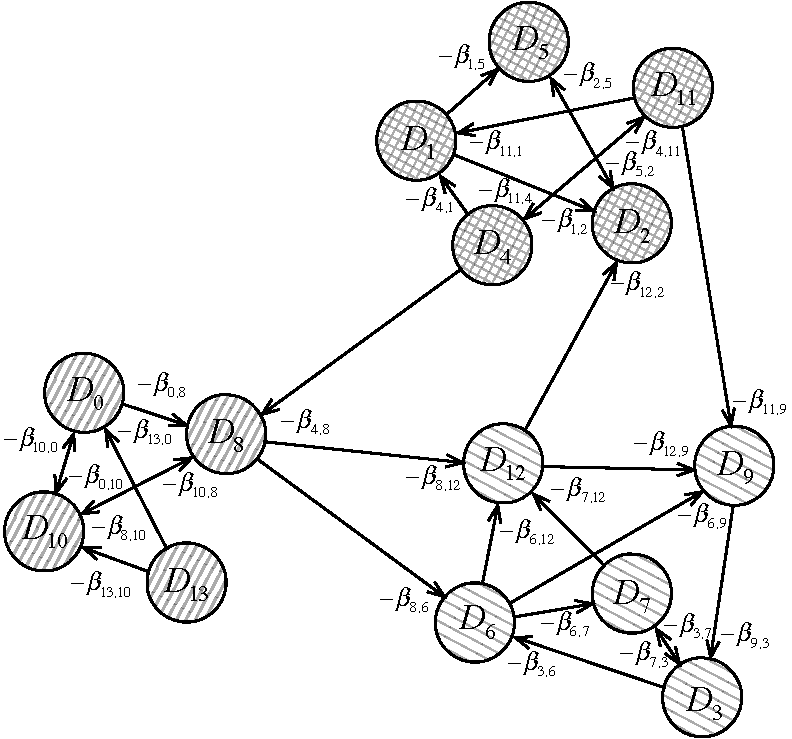
\includegraphics[width=.9\linewidth]{figs/graphConPartition}
  \caption{Graph construction and partition}
  \label{fig:graphConPartition}
\end{figure}


\subsection{Graph partition} \label{sec:graphPartition}

As mention in Section~\ref{sec:introduction}, many researcher use modularity for showing algorithm's performance or suggest heuristics that maximize modularity. The following equation is a formal mathematical representation of modularity;


\begin{equation} \label{eq:modularity}
	Q= \frac{1}{2m} \sum_{i,j} \Big[A_{ij} - \frac{k_{i}k_{j}}{2m}\Big] \delta(c_{i},c_{j})
\end{equation}

\noindent where $A_ij$ is the weight of the the edge $i$-$j$, $m=\frac{1}{2} \sum_{ij}A_{ij}$, $k_{i}=\sum_{j}A_{ij}$, $c_i$ is the community which node $i$ belong to, the $\delta$-function $\delta(u,v)$ is 1 if $u=v$ and 0 otherwise. The high modularity value means that the sum of the weight of intra-edge (edges within the community) is high but the sum of the weight of inter-edges (edges between communities) is low.

We regard that this community detection algorithm part is not our interest because well-known and well-performing algorithm already exist. Therefore, we use a library which is based on  Blondel et al.~\shortcite{Blondel2008} and can also directed and weighted graphs.


\subsection{Zone discovery} \label{sec:zoneDiscovery}

Our final interest is zones where members in the same community influence each other. We consider that there are specific zones where members share information about. For example, if a location is a popular place, a driver already know the information about that place before other members let the driver know it. On the contrary to this, there can be a location where a driver know well and the driver contribute his community's productivity.

To discover these zones, we suggest another regression model. For a community, we apply the following equation;

\begin{equation} \label{eq:zoneRegression}
	q_{z}= \alpha + \beta_{z}X_{z} + \epsilon
\end{equation}

\noindent where $q_{z}$ is queueing time at zone $z$ and $X_{z}$is a binary variable about any member's prior presence at zone $z$. As Section~\ref{sec:graphConstruction}, we use 10\% significance level and find zones whose $\beta_{z}$ is a negative value.

\section{Experiments} \label{sec:experiments}

In this section, we shows some meaningful results for each phrase in \ref{sec:comDectectionFramework}. The first phrase is about queueing time. Figure~\ref{fig:queueTimeDist} shows queueing time's distribution of sampled data, January 2009 after the filtering procedure. The distribution is very skewed, 50\% of queueing time is less than six minutes. It implies that most taxi drivers leave a location and find another location if they cannot pick up a new passenger in six minutes. 


\begin{figure} [h]
  \centering
  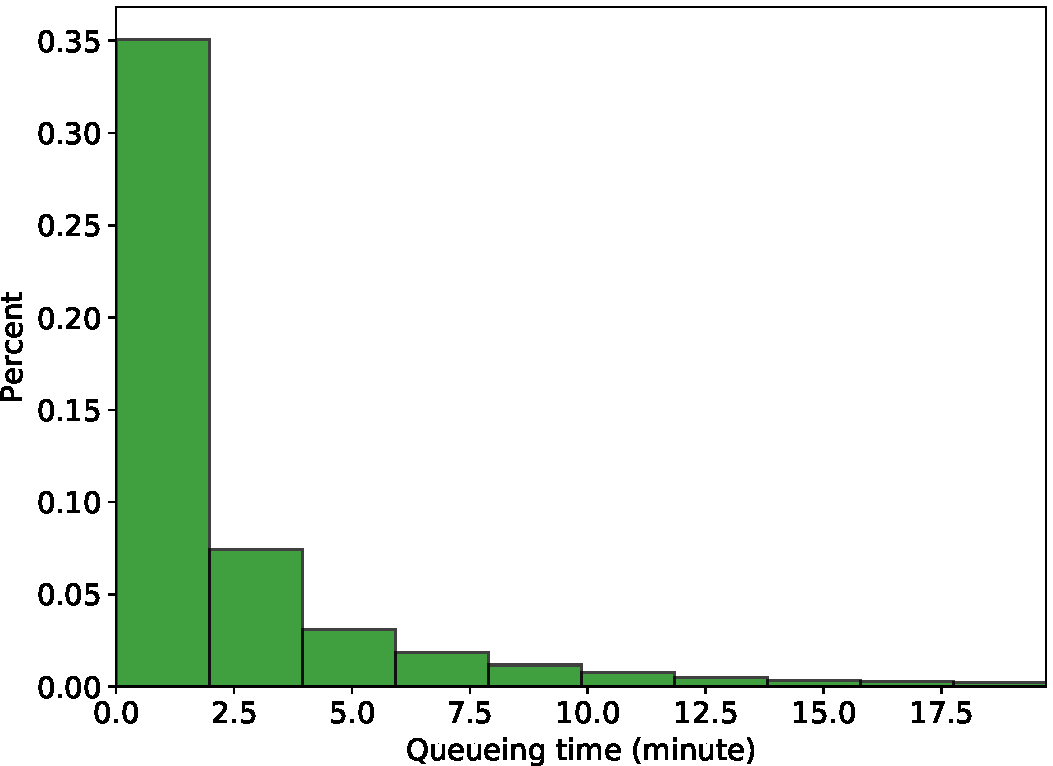
\includegraphics[width=.9\linewidth]{figs/queueTimeDist}
  \caption{Queueing time distribution}
  \label{fig:queueTimeDist}
\end{figure}


The second result we want to show is the regression model's result about relationships between drivers. To get enough number of instances, we collect each driver's all trips in a year. Table~\ref{tab:resultInfluenceRegression} shows the regression result of a driver whose ID is 12327. In the table, \emph{var} represents independent variable and each number in the row is other driver's ID (const represents the intercept, this can be regarded as the average queueing time of the driver). The number of instances is 176, the number of independent variables is 76 and  p-value of f-statistic is 0.005 which is less than 1\%. Among 76 drivers, the influence (\emph{coef}) of driver 33477 is statistically meaninful in terms of the significance level. Therefore, we build a edge which directs from driver 33477 to driver 12327 and whose weight is 1.486 minute.

\begin{table}[h]
	\caption{A result of regression model about driver 12327}
	\vspace{-0.3 cm}
	\begin{center}
		\begin{tabular}{c|rrrr}
		  	\emph{var} 	& \multicolumn{1}{c}{\emph{coef} }	& \multicolumn{1}{c}{\emph{std err}}	& \multicolumn{1}{c}{\emph{t-score}}	& \multicolumn{1}{c}{\emph{p-value}} \\
		  \hline
			const 	& 1.321 	& 0.213 	& 6.214 	& 0.000 \\
			272 		& -0.304 	& 0.524 	& -0.581 	& 0.562 \\
			345 		& -0.109 	& 0.585 	& -0.186 	& 0.853 \\
			33287 	& 0.470 	& 0.747 	& 0.629 	& 0.531 \\
			33477 	& -1.486 	& 0.517 	& -2.874 	& 0.005 \\
			2439 	& 0.223 	& 0.560 	& 0.398 	& 0.691 \\
			3332 	& 0.448 	& 0.570 	& 0.786 	& 0.434 \\
			3426 	& -1.312 	& 0.547 	& -2.396 	& 0.018 \\
			...			&				&				&				&		
		\end{tabular}
	\label{tab:resultInfluenceRegression}
	\end{center}
	\vspace{-0.3 cm}
\end{table}

After graph partition phrase, we check the number of members in a community and two statistics; 

\begin{itemize}
	\item \emph{tie-strength}: the sum of edges' weight over the number of members in the community
	\item \emph{contribution}: \emph{tie-strength} over the number of members in the community
\end{itemize}

\noindent \emph{contribution} is the proxy of the average amount of queue time the prior presence of other members decreases. With 2012 dataset, we find 68 communities, but most of them, especially big communities, shows low values in \emph{contribution}, less than one minutes. Table~\ref{tab:partitionResult} shows top eight communities in terms of \emph{contribution}. Following the our frame work, a contact of a member in community $C_6$ contributes 1.142 minutes reduction to other member's queueing time.

\begin{table}[h]
	\caption{A result of graph partition in 2012}
	\vspace{-0.3 cm}
	\begin{center}
		\begin{tabular}{c|rrrr}
		  	\emph{comName} 	& \multicolumn{1}{c}{\emph{numDrivers} }	& \multicolumn{1}{c}{\emph{tie-strength}}	& \multicolumn{1}{c}{\emph{contribution}} \\
		  \hline
			$C_1$ 	& 3 		& 9.643 	& 3.214 \\
			$C_2$ 	& 3 		& 6.221 	& 2.074 \\
			$C_3$ 	& 3 		& 5.060 	& 1.687 \\
			$C_4$ 	& 2 		& 2.903 	& 1.451 \\
			$C_5$ 	& 2 		& 2.588 	& 1.294 \\
			$C_6$ 	& 20	& 22.839 & 1.142 \\
			$C_7$ 	& 32 	& 31.502 & 0.984 \\
			$C_8$ 	& 2 		& 1.939 	& 0.969 \\
			... & & &
		\end{tabular}
	\label{tab:partitionResult}
	\end{center}
	\vspace{-0.3 cm}
\end{table}


\begin{figure} [h]
  \centering
  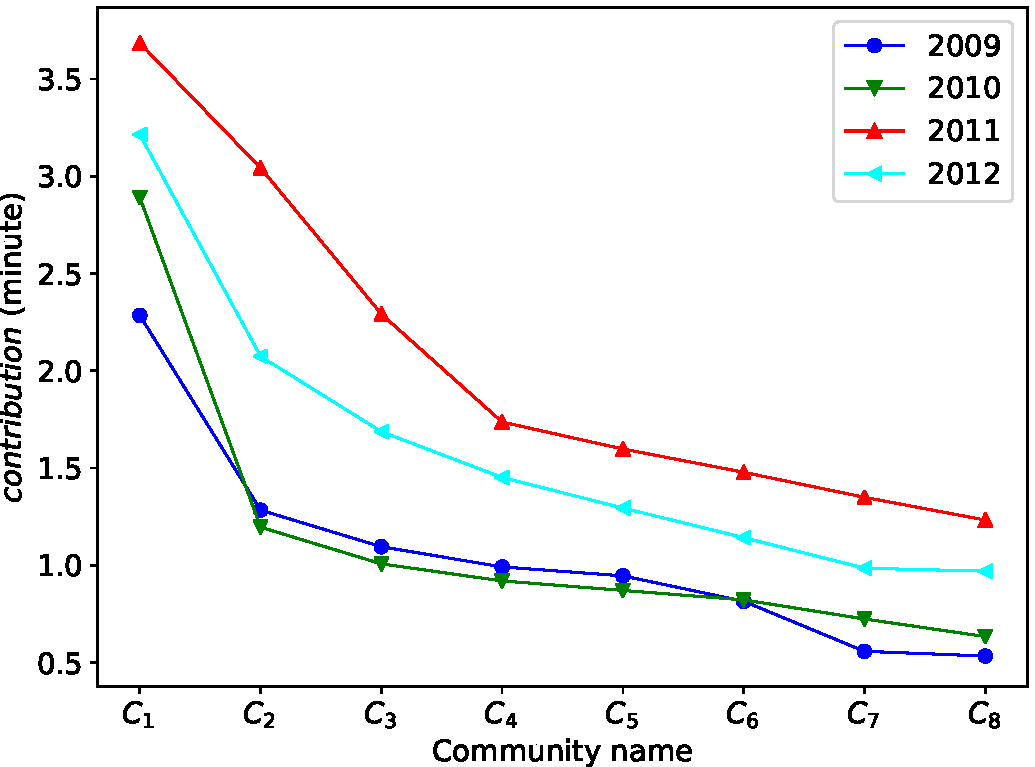
\includegraphics[width=.9\linewidth]{figs/yearContribution}
  \caption{Top eight communities contribution for each year}
  \label{fig:yearContribution}
\end{figure}

% 2009~2012 dataset
% Changes in contribution
%		before smart phone (2009) bigger community

% zoneRegression result
% zone discovery 
% Original and zoom in

\begin{figure} [h]
  \centering
  \includegraphics[width=.9\linewidth]{figs/zoneDiscovery}
  \caption{Top eight communities contribution for each year}
  \label{fig:zoneDiscovery}
\end{figure}


%49#15 -152.16, 3, 1048
%22#22 -110.76, 11, 1048
%41#16 -57.21, 16, 1048
% 40#16 -152.38, 288, 1048

\section{Discussions and Conclusions} \label{sec:discuCons}

% evolutions
% marginal influence
% parameters

% summary this research
%		contribution

% Future works
% non-single shift drivers



%% The file named.bst is a bibliography style file for BibTeX 0.99c
\bibliographystyle{named}
\bibliography{ijcai17}

\end{document}

